\section{第二次作业}
\noindent \textbf{AUTO2005 信号分析与处理（Signal Analysis and Processing）}
\vspace{0.5em}
\hrule
\vspace{1em}
\begin{center}
    \Large\textbf{第二次作业} \\
    \normalsize 2026年4月3日
\end{center}
\vspace{1em}
\noindent \textbf{【注意】} 作业交纸质版，注明题号，不需要抄题。所有题目请写出详细求解步骤，如使用函数的对称性等技巧化简求解过程，必须写出详细原因，例如：“因为函数是偶函数”、“奇函数，……”、“根据某某性质，……”等。如果完全不写求解过程步骤直接给出答案，将视情况扣分。该原则适用于本课程所有作业。部分作业题给了提示，但注意：考试不会给提示。
\vspace{1em}

% ==============================================
% 第1题 完整题目+详细解答
% ==============================================
\subsection{1. 连续时间周期信号傅里叶级数}
\subsubsection{(1) 三角傅里叶级数形式转换}
\textbf{题目：} 有一实值连续时间周期信号 \( f(t) \)，其基波周期为 \( T_1=8 \)，\( f(t) \) 的非零复指数傅里叶级数系数为 \( F_1=F_{-1}=2 \)，\( F_3=F_{-3}^*=4j \)，要求将 \( f(t) \) 表示成三角傅里叶级数形式。

\paragraph{求解步骤：}
\textcircled{1} 计算基波角频率：
\[
\omega_1 = \frac{2\pi}{T_1} = \frac{2\pi}{8} = \frac{\pi}{4} \ \mathrm{rad/s}
\]
\textcircled{2} 写出复指数傅里叶级数展开式：
\[
f(t) = \sum_{n=-\infty}^{\infty} F_n e^{jn\omega_1 t} = F_{-3}e^{-j3\omega_1 t} + F_{-1}e^{-j\omega_1 t} + F_1e^{j\omega_1 t} + F_3e^{j3\omega_1 t}
\]
代入已知系数（\( F_{-3} = (F_3)^* = -4j \)）：
\[
f(t) = -4j e^{-j\frac{3\pi}{4}t} + 2e^{-j\frac{\pi}{4}t} + 2e^{j\frac{\pi}{4}t} + 4j e^{j\frac{3\pi}{4}t}
\]
\textcircled{3} 利用欧拉公式化简为三角形式：
- 对 \( n=\pm1 \) 项：\( 2e^{j\frac{\pi}{4}t} + 2e^{-j\frac{\pi}{4}t} = 4\cos\left(\frac{\pi}{4}t\right) \)
- 对 \( n=\pm3 \) 项：
\[
\begin{aligned}
4j e^{j\frac{3\pi}{4}t} - 4j e^{-j\frac{3\pi}{4}t} &= 4j\left[\left(\cos\frac{3\pi}{4}t + j\sin\frac{3\pi}{4}t\right) - \left(\cos\frac{3\pi}{4}t - j\sin\frac{3\pi}{4}t\right)\right] \\
&= 4j \cdot 2j\sin\frac{3\pi}{4}t = -8\sin\left(\frac{3\pi}{4}t\right)
\end{aligned}
\]
\textcircled{4} 最终三角傅里叶级数：
\[
\boxed{f(t) = 4\cos\left(\frac{\pi}{4}t\right) - 8\sin\left(\frac{3\pi}{4}t\right)}
\]

\subsubsection{(2) 基波频率与复指数傅里叶级数}
\textbf{题目：} 对连续时间周期信号 \( x(t) = 2 + \cos\left(\frac{2\pi}{3}t\right) + 4\sin\left(\frac{5\pi}{3}t\right) \)，求 \( x(t) \) 的基波频率 \( \omega_1 \) 和复指数傅里叶级数系数 \( X_n \)，并给出复指数形式的傅里叶级数表达式。

\paragraph{求解步骤：}
\textcircled{1} 求基波角频率 \( \omega_1 \)：
将信号展开为复指数形式：
\[
\cos\left(\frac{2\pi}{3}t\right) = \frac{1}{2}e^{j\frac{2\pi}{3}t} + \frac{1}{2}e^{-j\frac{2\pi}{3}t}, \quad \sin\left(\frac{5\pi}{3}t\right) = \frac{1}{2j}e^{j\frac{5\pi}{3}t} - \frac{1}{2j}e^{-j\frac{5\pi}{3}t}
\]
各分量角频率为 \( 0, \pm\frac{2\pi}{3}, \pm\frac{5\pi}{3} \)，最大公约数为 \( \frac{\pi}{3} \)，因此：
\[
\boxed{\omega_1 = \frac{\pi}{3} \ \mathrm{rad/s}}
\]
基波周期 \( T_1 = \frac{2\pi}{\omega_1} = 6 \)。

\textcircled{2} 求复指数傅里叶系数 \( X_n \)：
根据 \( x(t) = \sum_{n=-\infty}^{\infty} X_n e^{jn\omega_1 t} = \sum_{n=-\infty}^{\infty} X_n e^{jn\frac{\pi}{3}t} \)，对比展开式得非零系数：
\[
\boxed{
\begin{aligned}
X_0 &= 2, \quad X_2 = X_{-2} = \frac{1}{2}, \\
X_5 &= -2j, \quad X_{-5} = 2j, \quad \text{其余} \ X_n=0
\end{aligned}
}
\]

\textcircled{3} 复指数傅里叶级数表达式：
\[
\boxed{x(t) = 2 + \frac{1}{2}e^{j\frac{2\pi}{3}t} + \frac{1}{2}e^{-j\frac{2\pi}{3}t} - 2j e^{j\frac{5\pi}{3}t} + 2j e^{-j\frac{5\pi}{3}t}}
\]

% ==============================================
% 第2题 完整题目+详细解答+2图一行
% ==============================================
\subsection{2. 利用对称性定性判断傅里叶级数频率分量}
\textbf{题目：} 利用信号的对称性，定性判断题图2-2中，各周期信号的傅里叶级数中所含有的频率分量。

\paragraph{对称性与傅里叶分量对应关系：}
\begin{itemize}
    \item \textbf{偶函数}：\( f(-t)=f(t) \)，仅含直流分量和余弦分量（$b_n=0$，无正弦分量）；
    \item \textbf{奇函数}：\( f(-t)=-f(t) \)，仅含正弦分量（$a_0=0,a_n=0$，无直流、余弦分量）；
    \item \textbf{半波对称信号}：\( f(t\pm T/2)=-f(t) \)，仅含奇次谐波分量，无偶次谐波和直流分量；
    \item \textbf{偶谐信号}：\( f(t\pm T/2)=f(t) \)，仅含偶次谐波分量。
\end{itemize}

\begin{figure}[htbp]
\centering
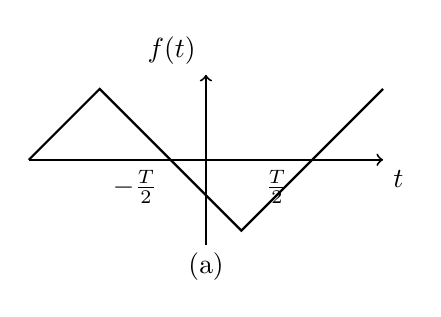
\begin{tikzpicture}[scale=0.9, line width=0.7pt]
% (a) 三角波（偶函数）
\draw[->] (-2.5,0) -- (2.5,0) node[below right] {$t$};
\draw[->] (0,-1.2) -- (0,1.2) node[above left] {$f(t)$};
\draw[thick] (-2.5,0) -- (-1.5,1) -- (-0.5,0) -- (0.5,-1) -- (1.5,0) -- (2.5,1);
\node at (-1,0) [below] {$-\frac{T}{2}$};
\node at (1,0) [below] {$\frac{T}{2}$};
\node at (0,-1.5) {(a)};
\end{tikzpicture}
\qquad
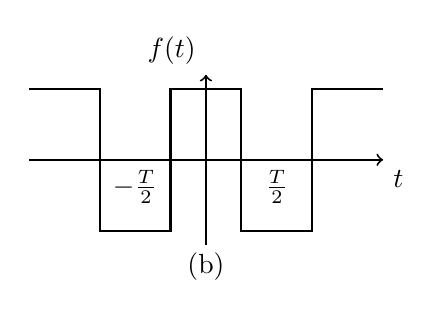
\begin{tikzpicture}[scale=0.9, line width=0.7pt]
% (b) 对称方波（奇函数+半波对称）
\draw[->] (-2.5,0) -- (2.5,0) node[below right] {$t$};
\draw[->] (0,-1.2) -- (0,1.2) node[above left] {$f(t)$};
\draw[thick] (-2.5,1) -- (-1.5,1) -- (-1.5,-1) -- (-0.5,-1) -- (-0.5,1) -- (0.5,1) -- (0.5,-1) -- (1.5,-1) -- (1.5,1) -- (2.5,1);
\node at (-1,0) [below] {$-\frac{T}{2}$};
\node at (1,0) [below] {$\frac{T}{2}$};
\node at (0,-1.5) {(b)};
\end{tikzpicture}
\caption{题图2-2 各周期信号波形}
\end{figure}

\begin{figure}[htbp]
\centering
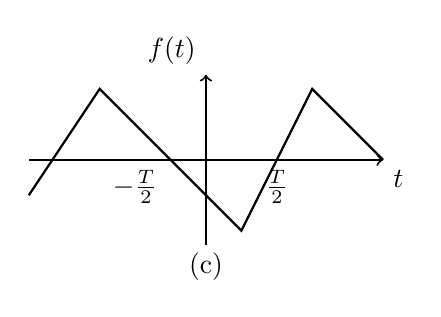
\begin{tikzpicture}[scale=0.9, line width=0.7pt]
% (c) 斜波（奇函数）
\draw[->] (-2.5,0) -- (2.5,0) node[below right] {$t$};
\draw[->] (0,-1.2) -- (0,1.2) node[above left] {$f(t)$};
\draw[thick] (-2.5,-0.5) -- (-1.5,1) -- (-0.5,0) -- (0.5,-1) -- (1.5,1) -- (2.5,0);
\node at (-1,0) [below] {$-\frac{T}{2}$};
\node at (1,0) [below] {$\frac{T}{2}$};
\node at (0,-1.5) {(c)};
\end{tikzpicture}
\qquad
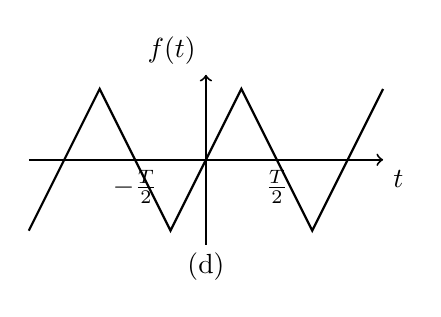
\begin{tikzpicture}[scale=0.9, line width=0.7pt]
% (d) 锯齿波（奇函数+半波对称）
\draw[->] (-2.5,0) -- (2.5,0) node[below right] {$t$};
\draw[->] (0,-1.2) -- (0,1.2) node[above left] {$f(t)$};
\draw[thick] (-2.5,-1) -- (-1.5,1) -- (-0.5,-1) -- (0.5,1) -- (1.5,-1) -- (2.5,1);
\node at (-1,0) [below] {$-\frac{T}{2}$};
\node at (1,0) [below] {$\frac{T}{2}$};
\node at (0,-1.5) {(d)};
\end{tikzpicture}
\caption{题图2-2 各周期信号波形（续）}
\end{figure}

\paragraph{各信号分量判断：}
\begin{enumerate}
    \item \textbf{图(a) 三角波}：$f(-t)=f(t)$ 为偶函数，且 $f(t+T/2)=f(t)$ 为偶谐信号，因此仅含直流分量和偶次余弦分量，无正弦分量、奇次谐波分量；
    \item \textbf{图(b) 方波}：$f(-t)=-f(t)$ 为奇函数，且 $f(t+T/2)=-f(t)$ 为半波对称信号，因此仅含奇次正弦分量，无直流分量、余弦分量、偶次谐波分量；
    \item \textbf{图(c) 斜波}：$f(-t)=-f(t)$ 为奇函数，无半波对称性，因此仅含所有次正弦分量，无直流分量、余弦分量；
    \item \textbf{图(d) 锯齿波}：$f(-t)=-f(t)$ 为奇函数，且 $f(t+T/2)=-f(t)$ 为半波对称信号，因此仅含奇次正弦分量，无直流分量、余弦分量、偶次谐波分量。
\end{enumerate}

% ==============================================
% 第3题 完整题目+详细解答
% ==============================================
\subsection{3. 周期三角波信号的傅里叶级数}
\textbf{题目：} 已知一个如题图2-3所示的周期三角波信号 \( f(t) \)：
(1) 求 \( f(t) \) 的傅里叶级数系数 \( a_0, a_n, b_n \)，并基于此给出三角傅里叶级数展开式，画出基于 \( c_n \) 的幅度频谱图（提示：$c_n$ 非负，简要分析该信号相角 \( \varphi_n \) 的取值）；
(2) 将 \( f(t) \) 左移 \( T/4 \)，求新信号的三角傅里叶级数表达式。

\begin{figure}[htbp]
\centering
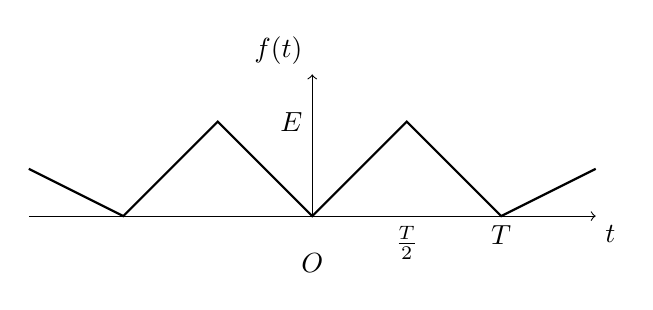
\begin{tikzpicture}[scale=1.2]
\draw[->] (-3,0) -- (3,0) node[below right] {$t$};
\draw[->] (0,0) -- (0,1.5) node[above left] {$f(t)$};
\draw[thick] (-3,0.5) -- (-2,0) -- (-1,1) -- (0,0) -- (1,1) -- (2,0) -- (3,0.5);
\node at (1,0) [below] {$\frac{T}{2}$};
\node at (2,0) [below] {$T$};
\node at (0,1) [left] {$E$};
\node at (0,-0.5) {$O$};
\end{tikzpicture}
\caption{题图2-3 周期三角波信号}
\end{figure}

\subsubsection{(1) 傅里叶级数系数与展开式}
\paragraph{步骤1：信号表达式（一个周期 \( [-T/2,T/2] \)）}
\[
f(t) =
\begin{cases}
\frac{2E}{T}t + E, & t\in[-T/2,0] \\
-\frac{2E}{T}t + E, & t\in[0,T/2]
\end{cases}
\]
\( f(t) \) 为偶函数，故 \( b_n=0 \ (\forall n) \)。

\paragraph{步骤2：求 \( a_0 \)}
\[
a_0 = \frac{2}{T}\int_{-T/2}^{T/2} f(t)dt = \frac{2}{T}\left(\int_{-T/2}^0 \left(\frac{2E}{T}t+E\right)dt + \int_0^{T/2} \left(-\frac{2E}{T}t+E\right)dt\right) = E
\]
直流分量 \( \frac{a_0}{2} = \frac{E}{2} \)。

\paragraph{步骤3：求 \( a_n \)}
\[
\begin{aligned}
a_n &= \frac{2}{T}\int_{-T/2}^{T/2} f(t)\cos(n\omega_1 t)dt = \frac{4}{T}\int_0^{T/2} \left(-\frac{2E}{T}t+E\right)\cos\left(\frac{2\pi n}{T}t\right)dt \\
&= \frac{4E}{\pi^2 n^2}\sin^2\left(\frac{n\pi}{2}\right)
\end{aligned}
\]
因此：
\[
\boxed{
a_n =
\begin{cases}
0, & n\text{为偶数} \\
\frac{4E}{\pi^2 n^2}, & n\text{为奇数}
\end{cases}, \quad b_n=0 \ (\forall n)
}
\]

\paragraph{步骤4：三角傅里叶级数展开式}
\[
\boxed{f(t) = \frac{E}{2} + \sum_{k=1}^{\infty} \frac{4E}{\pi^2 (2k-1)^2} \cos\left(\frac{2\pi(2k-1)}{T}t\right)}
\]

\paragraph{步骤5：幅度频谱与相位分析}
复指数系数 \( c_n = \frac{a_n - jb_n}{2} = \frac{a_n}{2} \)，因此：
- 幅度 \( |c_n| = \frac{a_n}{2} \)，非负实数；
- 相位 \( \varphi_n = 0 \)（$c_n$ 为正实数，无相位偏移）。

幅度谱：
\[
|c_n| =
\begin{cases}
\frac{E}{2}, & n=0 \\
0, & n\text{为偶数}, n\neq0 \\
\frac{2E}{\pi^2 n^2}, & n\text{为奇数}
\end{cases}
\]

\subsubsection{(2) 左移 \( T/4 \) 后的三角傅里叶级数}
信号左移 \( T/4 \) 后，新信号 \( g(t) = f(t+T/4) \)，根据傅里叶级数时移性质：
\[
g(t) = \frac{E}{2} + \sum_{n=1}^{\infty} a_n \cos\left(n\omega_1\left(t+\frac{T}{4}\right)\right) = \frac{E}{2} + \sum_{n=1}^{\infty} a_n \cos\left(n\omega_1 t + \frac{n\pi}{2}\right)
\]
代入 \( a_n \) 表达式：
\[
\boxed{g(t) = \frac{E}{2} + \sum_{k=1}^{\infty} \frac{4E}{\pi^2 (2k-1)^2} \cos\left(\frac{2\pi(2k-1)}{T}t + \frac{(2k-1)\pi}{2}\right)}
\]

% ==============================================
% 第4题 完整题目+详细解答
% ==============================================
\subsection{4. 半波余弦信号的三角傅里叶级数}
\textbf{题目：} 求题图2-4所示半波余弦信号的三角傅里叶级数。若 \( E=10\mathrm{V} \)，\( f=10\mathrm{kHz} \)，基于 \( c_n \) 画出该信号的幅度谱，要求横轴对应频率的单位为Hz（提示：$c_n$ 非负；注意单位）。

\begin{figure}[htbp]
\centering
\begin{tikzpicture}[scale=1.2]
\draw[->] (-3,0) -- (3,0) node[below right] {$t$};
\draw[->] (0,0) -- (0,1.3) node[above left] {$f(t)$};
\draw[thick] (-3,0) -- (-1.5,0);
\draw[thick] plot[domain=-1.5:1.5] (\x, {cos(\x*60)});
\draw[thick] (1.5,0) -- (3,0);
\node at (-1.5,0) [below] {$-\frac{T}{4}$};
\node at (1.5,0) [below] {$\frac{T}{4}$};
\node at (-3,0) [below] {$-T$};
\node at (3,0) [below] {$T$};
\node at (0,1) [left] {$E$};
\node at (0,-0.5) {$O$};
\end{tikzpicture}
\caption{题图2-4 半波余弦信号}
\end{figure}

\paragraph{求解步骤：}
\textcircled{1} 信号参数：周期 \( T = \frac{1}{f} = 10^{-4}\mathrm{s} \)，基波角频率 \( \omega_1 = 2\pi f = 2\pi\times10^4 \ \mathrm{rad/s} \)，一个周期 \( [-T/2,T/2] \) 内表达式：
\[
f(t) =
\begin{cases}
E\cos(\omega_1 t), & |t| < T/4 \\
0, & T/4 < |t| < T/2
\end{cases}
\]
\( f(t) \) 为偶函数，故 \( b_n=0 \)。

\textcircled{2} 求傅里叶系数：
\[
a_0 = \frac{2}{T}\int_{-T/2}^{T/2} f(t)dt = \frac{2E}{T}\int_{-T/4}^{T/4} \cos(\omega_1 t)dt = \frac{2E}{\pi}
\]
\[
\begin{aligned}
a_n &= \frac{2}{T}\int_{-T/4}^{T/4} E\cos(\omega_1 t)\cos(n\omega_1 t)dt \\
&= \frac{2E}{\pi}\cdot\frac{(-1)^{n+1}}{n^2-1}, \quad n\neq1 \\
a_1 &= \frac{2E}{T}\int_{-T/4}^{T/4} \cos^2(\omega_1 t)dt = \frac{E}{2}
\end{aligned}
\]

\textcircled{3} 三角傅里叶级数展开式：
\[
\boxed{f(t) = \frac{E}{\pi} + \frac{E}{2}\cos(\omega_1 t) + \sum_{n=2}^{\infty} \frac{2E(-1)^{n+1}}{\pi(n^2-1)} \cos(n\omega_1 t)}
\]
代入 \( E=10\mathrm{V}, f=10\mathrm{kHz} \)：
\[
f(t) = \frac{10}{\pi} + 5\cos(2\pi\times10^4 t) + \sum_{n=2}^{\infty} \frac{20(-1)^{n+1}}{\pi(n^2-1)} \cos(2\pi n\times10^4 t)
\]

\textcircled{4} 幅度谱（单位Hz）：
复指数系数 \( c_n = \frac{a_n}{2} \)，对应频率 \( f_n = nf = n\times10\mathrm{kHz} \)，幅度：
\[
|c_0| = \frac{10}{\pi} \approx 3.18\mathrm{V}, \quad |c_1| = 2.5\mathrm{V}, \quad |c_n| = \frac{10(-1)^{n+1}}{\pi(n^2-1)}, \ n\geq2
\]

% ==============================================
% 第5题 完整题目+详细解答+2图一行
% ==============================================
\subsection{5. 利用傅里叶变换定义式求傅里叶变换}
\textbf{题目：} 利用傅里叶变换的定义式，求题图2-5 (a)、(b)所示信号的傅里叶变换。

\begin{figure}[htbp]
\centering
\begin{tikzpicture}[scale=1.1]
% (a) 单周正弦脉冲
\draw[->] (-0.5,0) -- (2.5,0) node[below right] {$t$};
\draw[->] (0,-1.3) -- (0,1.3) node[above left] {$f(t)$};
\draw[thick] plot[domain=0:2] (\x, {sin(\x*90)});
\node at (2,0) [below] {$T$};
\node at (0.8,1.2) {$E$};
\node at (1,-1.5) {(a) 单周正弦脉冲};
\end{tikzpicture}
\qquad
\begin{tikzpicture}[scale=1.1]
% (b) 矩形脉冲组合
\draw[->] (-2,0) -- (2,0) node[below right] {$t$};
\draw[->] (0,-1.3) -- (0,1.3) node[above left] {$f(t)$};
\draw[thick] (-1.5,1) -- (0,1) -- (0,-1) -- (1.5,-1);
\node at (-1.5,0) [below] {$-\tau$};
\node at (1.5,0) [below] {$\tau$};
\node at (0,1.2) {$E$};
\node at (0,-1.2) {$-E$};
\node at (0,-1.5) {(b) 矩形脉冲组合};
\end{tikzpicture}
\caption{题图2-5 非周期信号}
\end{figure}

傅里叶变换定义式：
\[
F(j\omega) = \int_{-\infty}^{\infty} f(t)e^{-j\omega t}dt
\]

\subsubsection{(a) 单周正弦脉冲}
信号表达式（\( \omega_0 = \frac{2\pi}{T} \)）：
\[
f(t) =
\begin{cases}
E\sin(\omega_0 t), & 0\leq t\leq T \\
0, & \text{其他}
\end{cases}
\]
\[
\begin{aligned}
F(j\omega) &= \int_0^T E\sin(\omega_0 t)e^{-j\omega t}dt \\
&= \frac{E}{2j}\int_0^T \left(e^{j\omega_0 t} - e^{-j\omega_0 t}\right)e^{-j\omega t}dt \\
&= \frac{E\omega_0(1-e^{-j\omega T})}{\omega_0^2 - \omega^2}
\end{aligned}
\]
\[
\boxed{F(j\omega) = \frac{E\cdot\frac{2\pi}{T}\left(1-e^{-j\omega T}\right)}{\left(\frac{2\pi}{T}\right)^2 - \omega^2}}
\]

\subsubsection{(b) 双极性矩形脉冲}
信号表达式：
\[
f(t) =
\begin{cases}
E, & -\tau < t < 0 \\
-E, & 0 < t < \tau \\
0, & \text{其他}
\end{cases}
\]
\[
\begin{aligned}
F(j\omega) &= \int_{-\tau}^0 E e^{-j\omega t}dt + \int_0^\tau (-E) e^{-j\omega t}dt \\
&= E\cdot\frac{1-e^{j\omega\tau}}{-j\omega} - E\cdot\frac{e^{-j\omega\tau}-1}{-j\omega} \\
&= \frac{2E j(1-\cos(\omega\tau))}{\omega}
\end{aligned}
\]
\[
\boxed{F(j\omega) = j\frac{2E(1-\cos\omega\tau)}{\omega}}
\]